\begin{frame}
    \frametitle{Giróscopo o Giroscopio}
    \scriptsize
    \begin{center}
        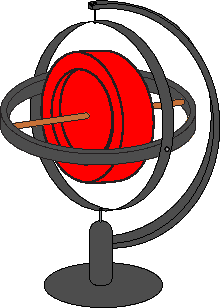
\includegraphics[width=0.2\columnwidth]{images/gyroscope.pdf}
    \end{center}

    \begin{block}{Principio de funcionamiento}
        Un giróscopo es todo cuerpo simétrico en Rotación a una velocidad suficiente como para experimentar los efectos giroscópicos.

        Los giroscopios son dispositivos que miden o mantienen el movimiento de rotación.
    \end{block}

    \begin{itemize}
        \item Introceptivo
        \item Pasivo
        \item Mide Velocidad Angular
        \item Unidad de medición $\si{\degree\second}$ o Revoluciones por Minuto (RPM)
    \end{itemize}

    \note{https://answeringatpl.com/instrumentation/gyroscopic-principles/\\
          https://www.5hertz.com/index.php?route=tutoriales/tutorial&tutorial_id=13
      }

\end{frame}

\begin{frame}
    \frametitle{Giróscopo: Pricipios giroscópicos}
    \note{https://www.youtube.com/watch?v=nhNg-8RSuKY}
    \scriptsize

    \begin{block}{Rigidez en el espacio}
        Al rotar, un giróscopo permanece en una posición fija en su plano de rotación, independientemente del movimiento de los soportes o el marco.

        La cantidad de rigidez que presenta el giróscopo es directamente proporcional a su velocidad de rotación (RPM) y su momento de inercia.
        Mayor velocidad de rotación, entonces mayor rigidez en el espacio.
        Mayor masa y radio efectivo, entonces mayor rigidez en el espacio.
    \end{block}

    \begin{block}{Precesión}
    Toda fuerza aplicada perpendicularmente sobre el plano de rotación de un giróscopo se verá reflejada a $\SI{90}{\degree}$ en el sentido de la rotación.

    La magnitud de la precesión que pesenta el giróscopo es directamente proporcional a la fuerza aplicada e inversamente proporcional a la velocidad de rotación (RPM).

    \begin{figure}[!h]
        \centering
        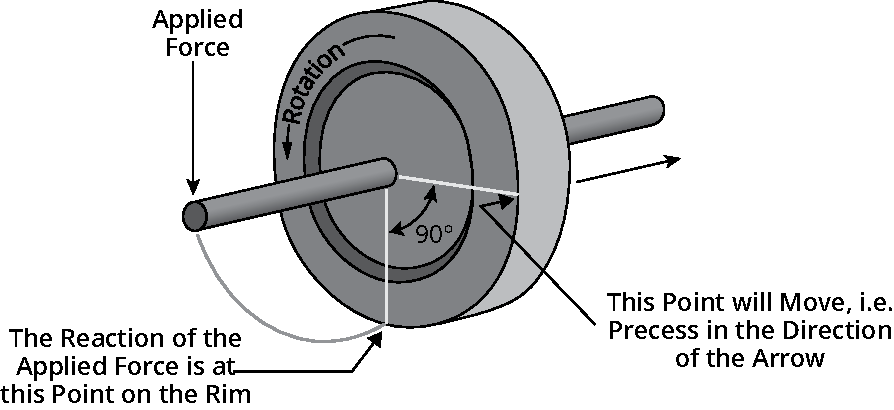
\includegraphics[width=0.4\columnwidth]{images/gyroscope_precession.pdf}
    \end{figure}
\end{block}

\note{Un trompo es un giróscopo! cuando esta por caerse muestra el efecto de precesión. La fuerza que se le aplica es la de la gravedad y hace que se mueva de realizando una circunsferencia con su eje.}
\end{frame}


\begin{frame}
    \frametitle{Giróscopo MEMS (Microelectromechanical Systems)}
    \note{https://www.analog.com/en/technical-articles/mems-gyroscope-provides-precision-inertial-sensing.html}
    \footnotesize
    \begin{block}{Principio de Funcionamiento}
        Los giroscopios MEMS utilizan la fuerza de Coriolis, la fuerza tangencial experimentada por un objeto giratorio en movimiento radial.
    \end{block}


    \begin{figure}[!h]
        \centering
        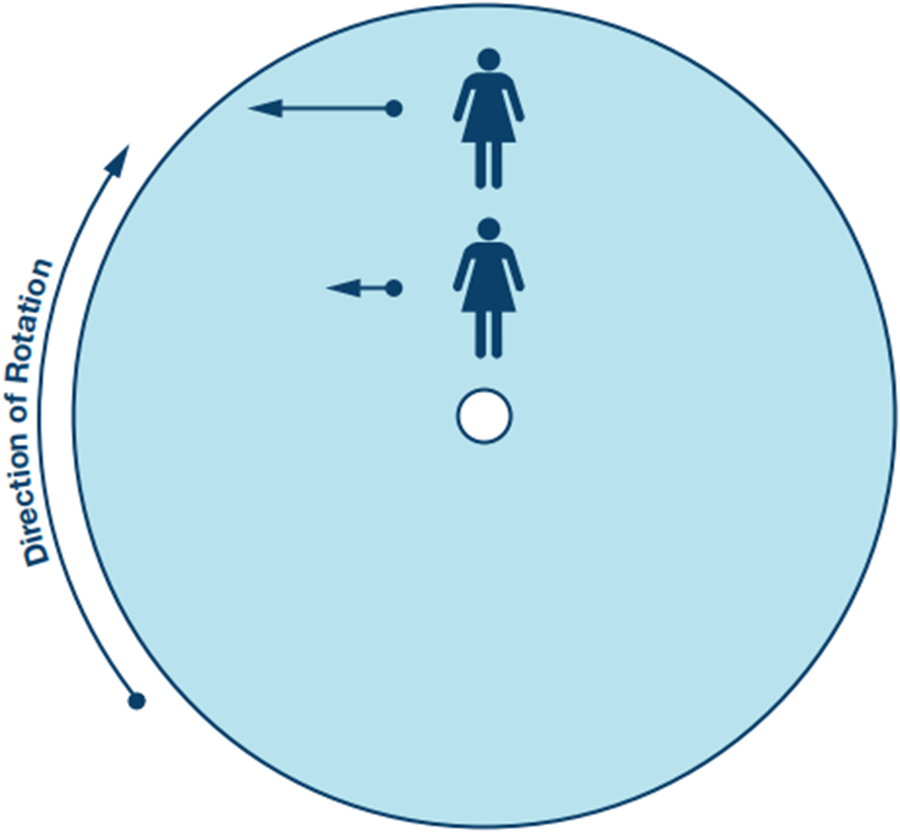
\includegraphics[width=0.2\columnwidth]{images/gyroscope_mems_1.png}
    \end{figure}

    Ejemplo de aceleración de Coriolis. Una persona que se mueve hacia el norte hacia el borde exterior de una plataforma giratoria debe aumentar el componente de velocidad hacia el oeste (flechas azules) para mantener un rumbo hacia el norte. La aceleración requerida es la aceleración de Coriolis.

    \note{Considérese parado en una plataforma giratoria, cerca del centro. Su velocidad relativa al suelo se muestra como la longitud de la flecha azul. Si tuviera que moverse a un punto cerca del borde exterior de la plataforma, su velocidad aumentaría en relación con el suelo, como lo indica la flecha azul más larga. La tasa de aumento de su velocidad tangencial, causada por su velocidad radial, es la aceleración de Coriolis.}

    \note{MEMS (sistemas microelectromecánicos) giroscopios son pequeños sensores, de bajo costo para medir la velocidad angular.  El sensor MEMS dentro de un giroscopio es muy pequeño (entre 1 a 100 micrómetros, el tamaño de un cabello humano).}

\end{frame}

\begin{frame}
    \frametitle{Giróscopo MEMS (Microelectromechanical Systems)}
    \footnotesize
    \note{https://www.analog.com/en/technical-articles/mems-gyroscope-provides-precision-inertial-sensing.html}

    Cuando se hace girar el giróscopo, una pequeña masa de resonancia se desplaza con los cambios de velocidad angular. Este movimiento se convierte en señales eléctricas de muy bajas corrientes que se pueden amplificar para ser leídas por un microcontrolador.

    \begin{figure}[!h]
        \centering
        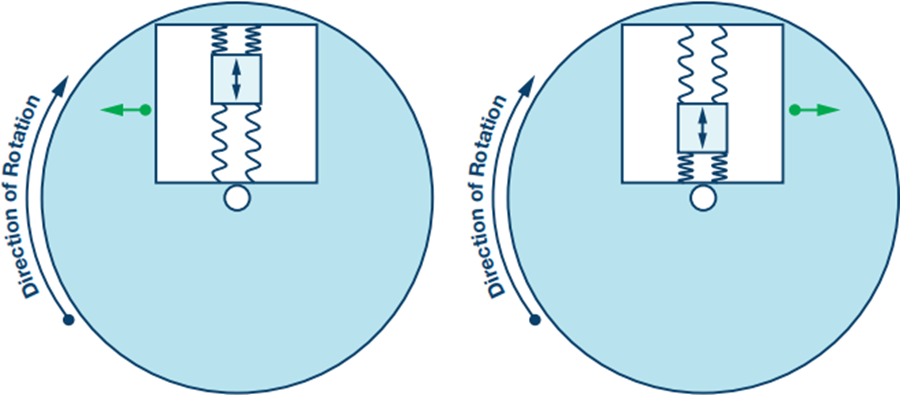
\includegraphics[width=0.4\columnwidth]{images/gyroscope_mems_2.png}
    \end{figure}

    Cuando la masa resonante se mueve hacia el borde exterior de la rotación, se acelera hacia la derecha y ejerce sobre el marco una fuerza de reacción hacia la izquierda. Cuando se mueve hacia el centro de la rotación, ejerce una fuerza hacia la derecha, como lo indican las flechas verdes.
\end{frame}

\begin{frame}
    \frametitle{Giróscopo MEMS (Microelectromechanical Systems)}
    \scriptsize
    \note{https://www.analog.com/en/technical-articles/mems-gyroscope-provides-precision-inertial-sensing.html}

    \begin{figure}[!h]
        \centering
        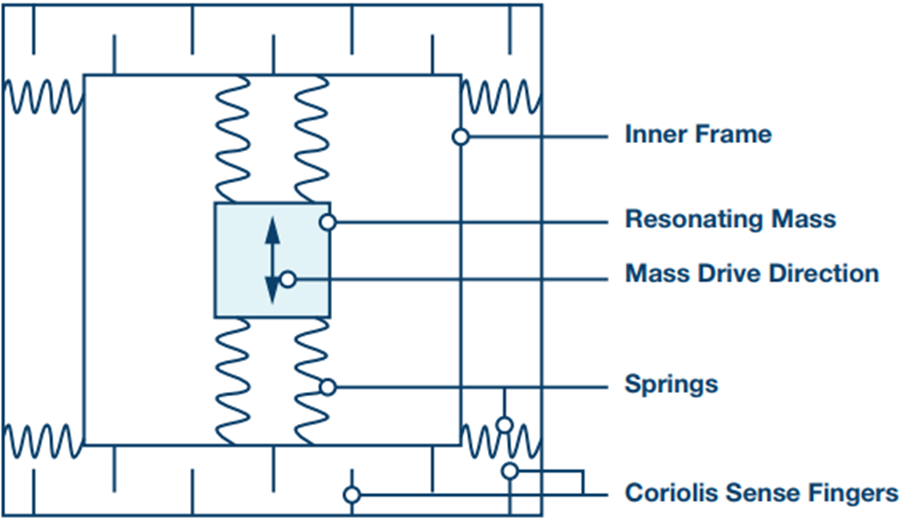
\includegraphics[width=0.2\columnwidth]{images/gyroscope_mems_structure.png}
    \end{figure}


    Para medir la aceleración de Coriolis, el marco que contiene la masa resonante está sujeto al sustrato por resortes a $\SI{90}{\degree}$ en relación con el movimiento resonante, como se muestra en la figura. Esta figura también muestra los dedos de detección de Coriolis que se utilizan para detectar el desplazamiento de la trama mediante transducción capacitiva en respuesta a la fuerza ejercida por la masa.

    \begin{figure}[!h]
        \centering
        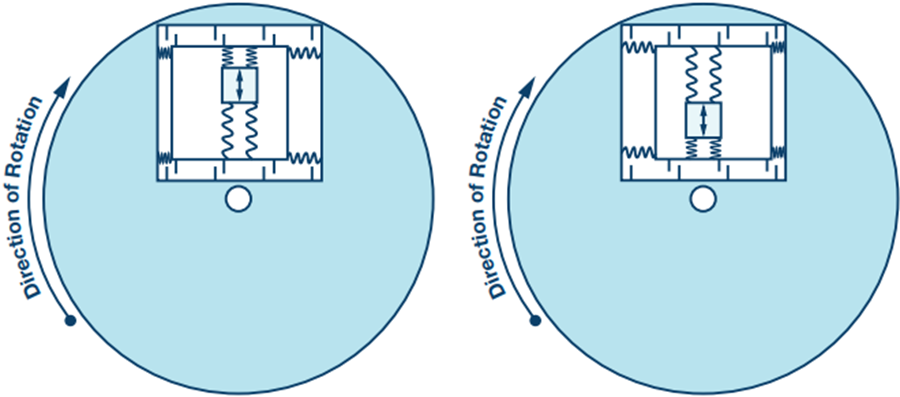
\includegraphics[width=0.3\columnwidth]{images/gyroscope_mems_3.png}
    \end{figure}

    A medida que la masa resonante se mueve y la superficie en la que está montado el giroscopio gira, la masa y su marco experimentan la aceleración de Coriolis y se trasladan 90 ° del movimiento vibratorio. A medida que aumenta la velocidad de rotación, también cambia el desplazamiento de la masa y la señal derivada de la capacitancia correspondiente.
\end{frame}



\begin{frame}
    \frametitle{Acelerómetro}
    
    \begin{figure}[!h]
    	\centering
    	\subfloat[]
    	{
    		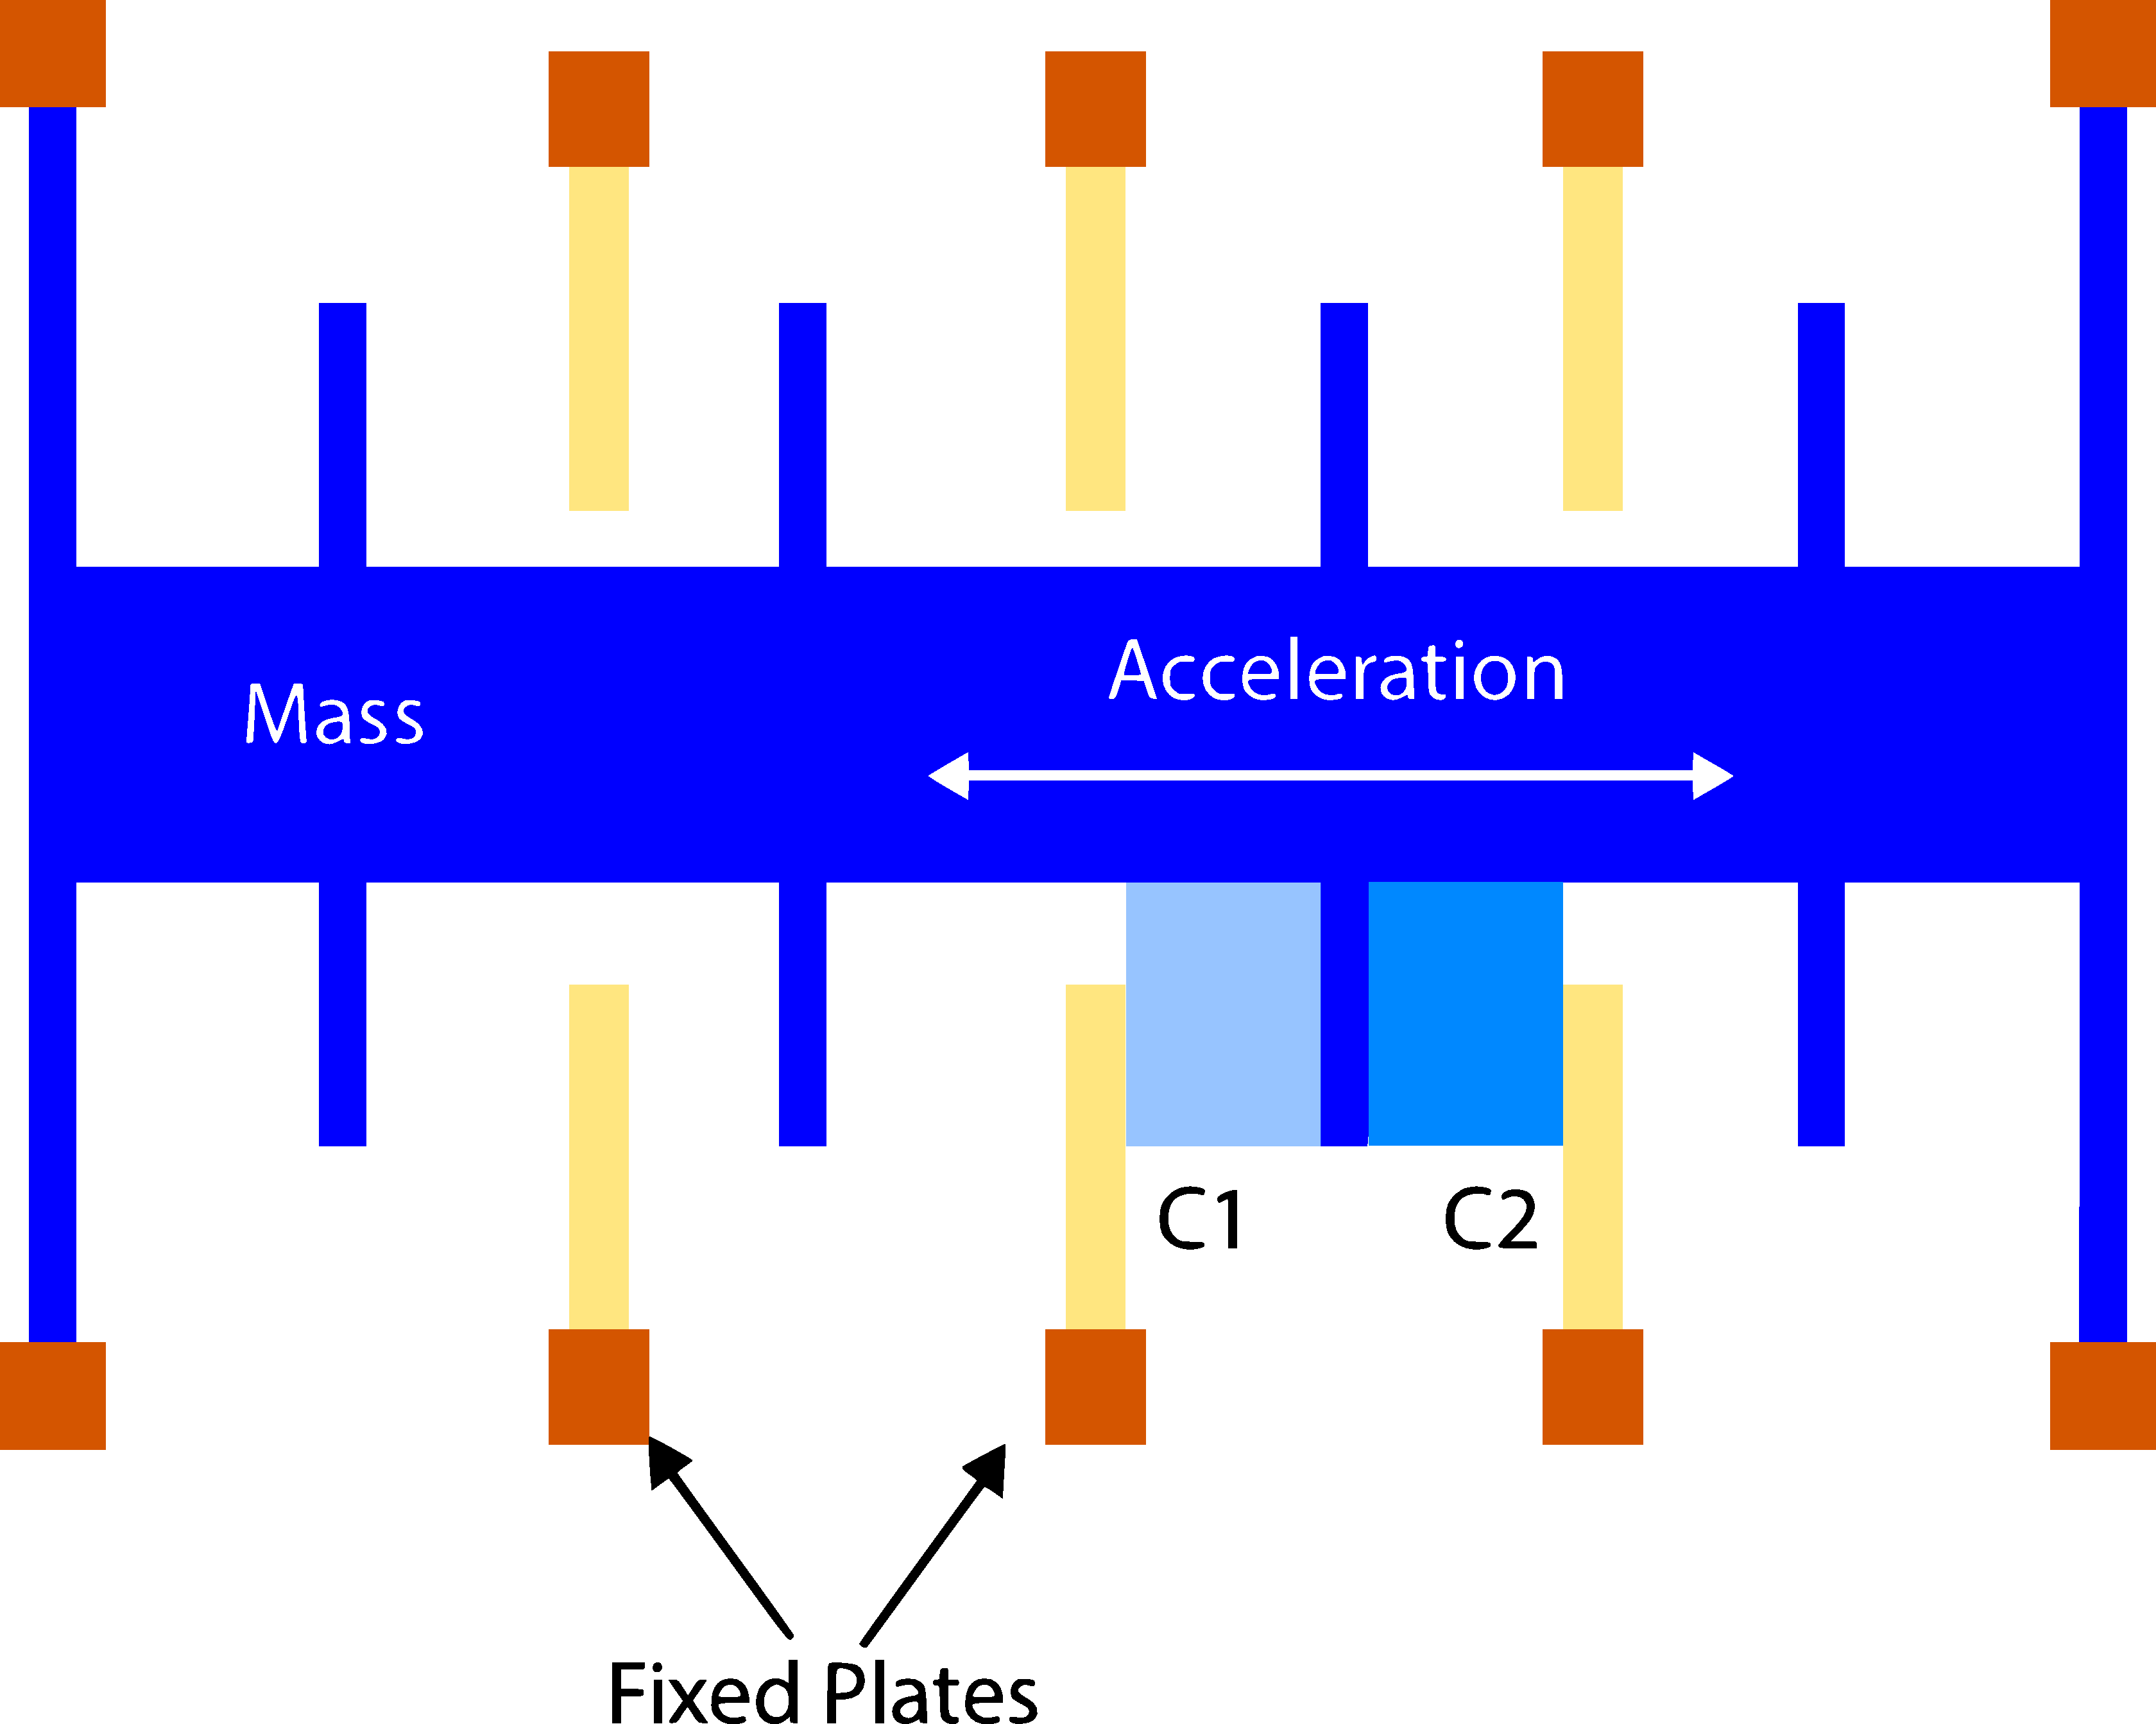
\includegraphics[width=0.2\columnwidth]{images/accelerometer_mems.pdf}
    	}
    	\subfloat[]
    	{
    		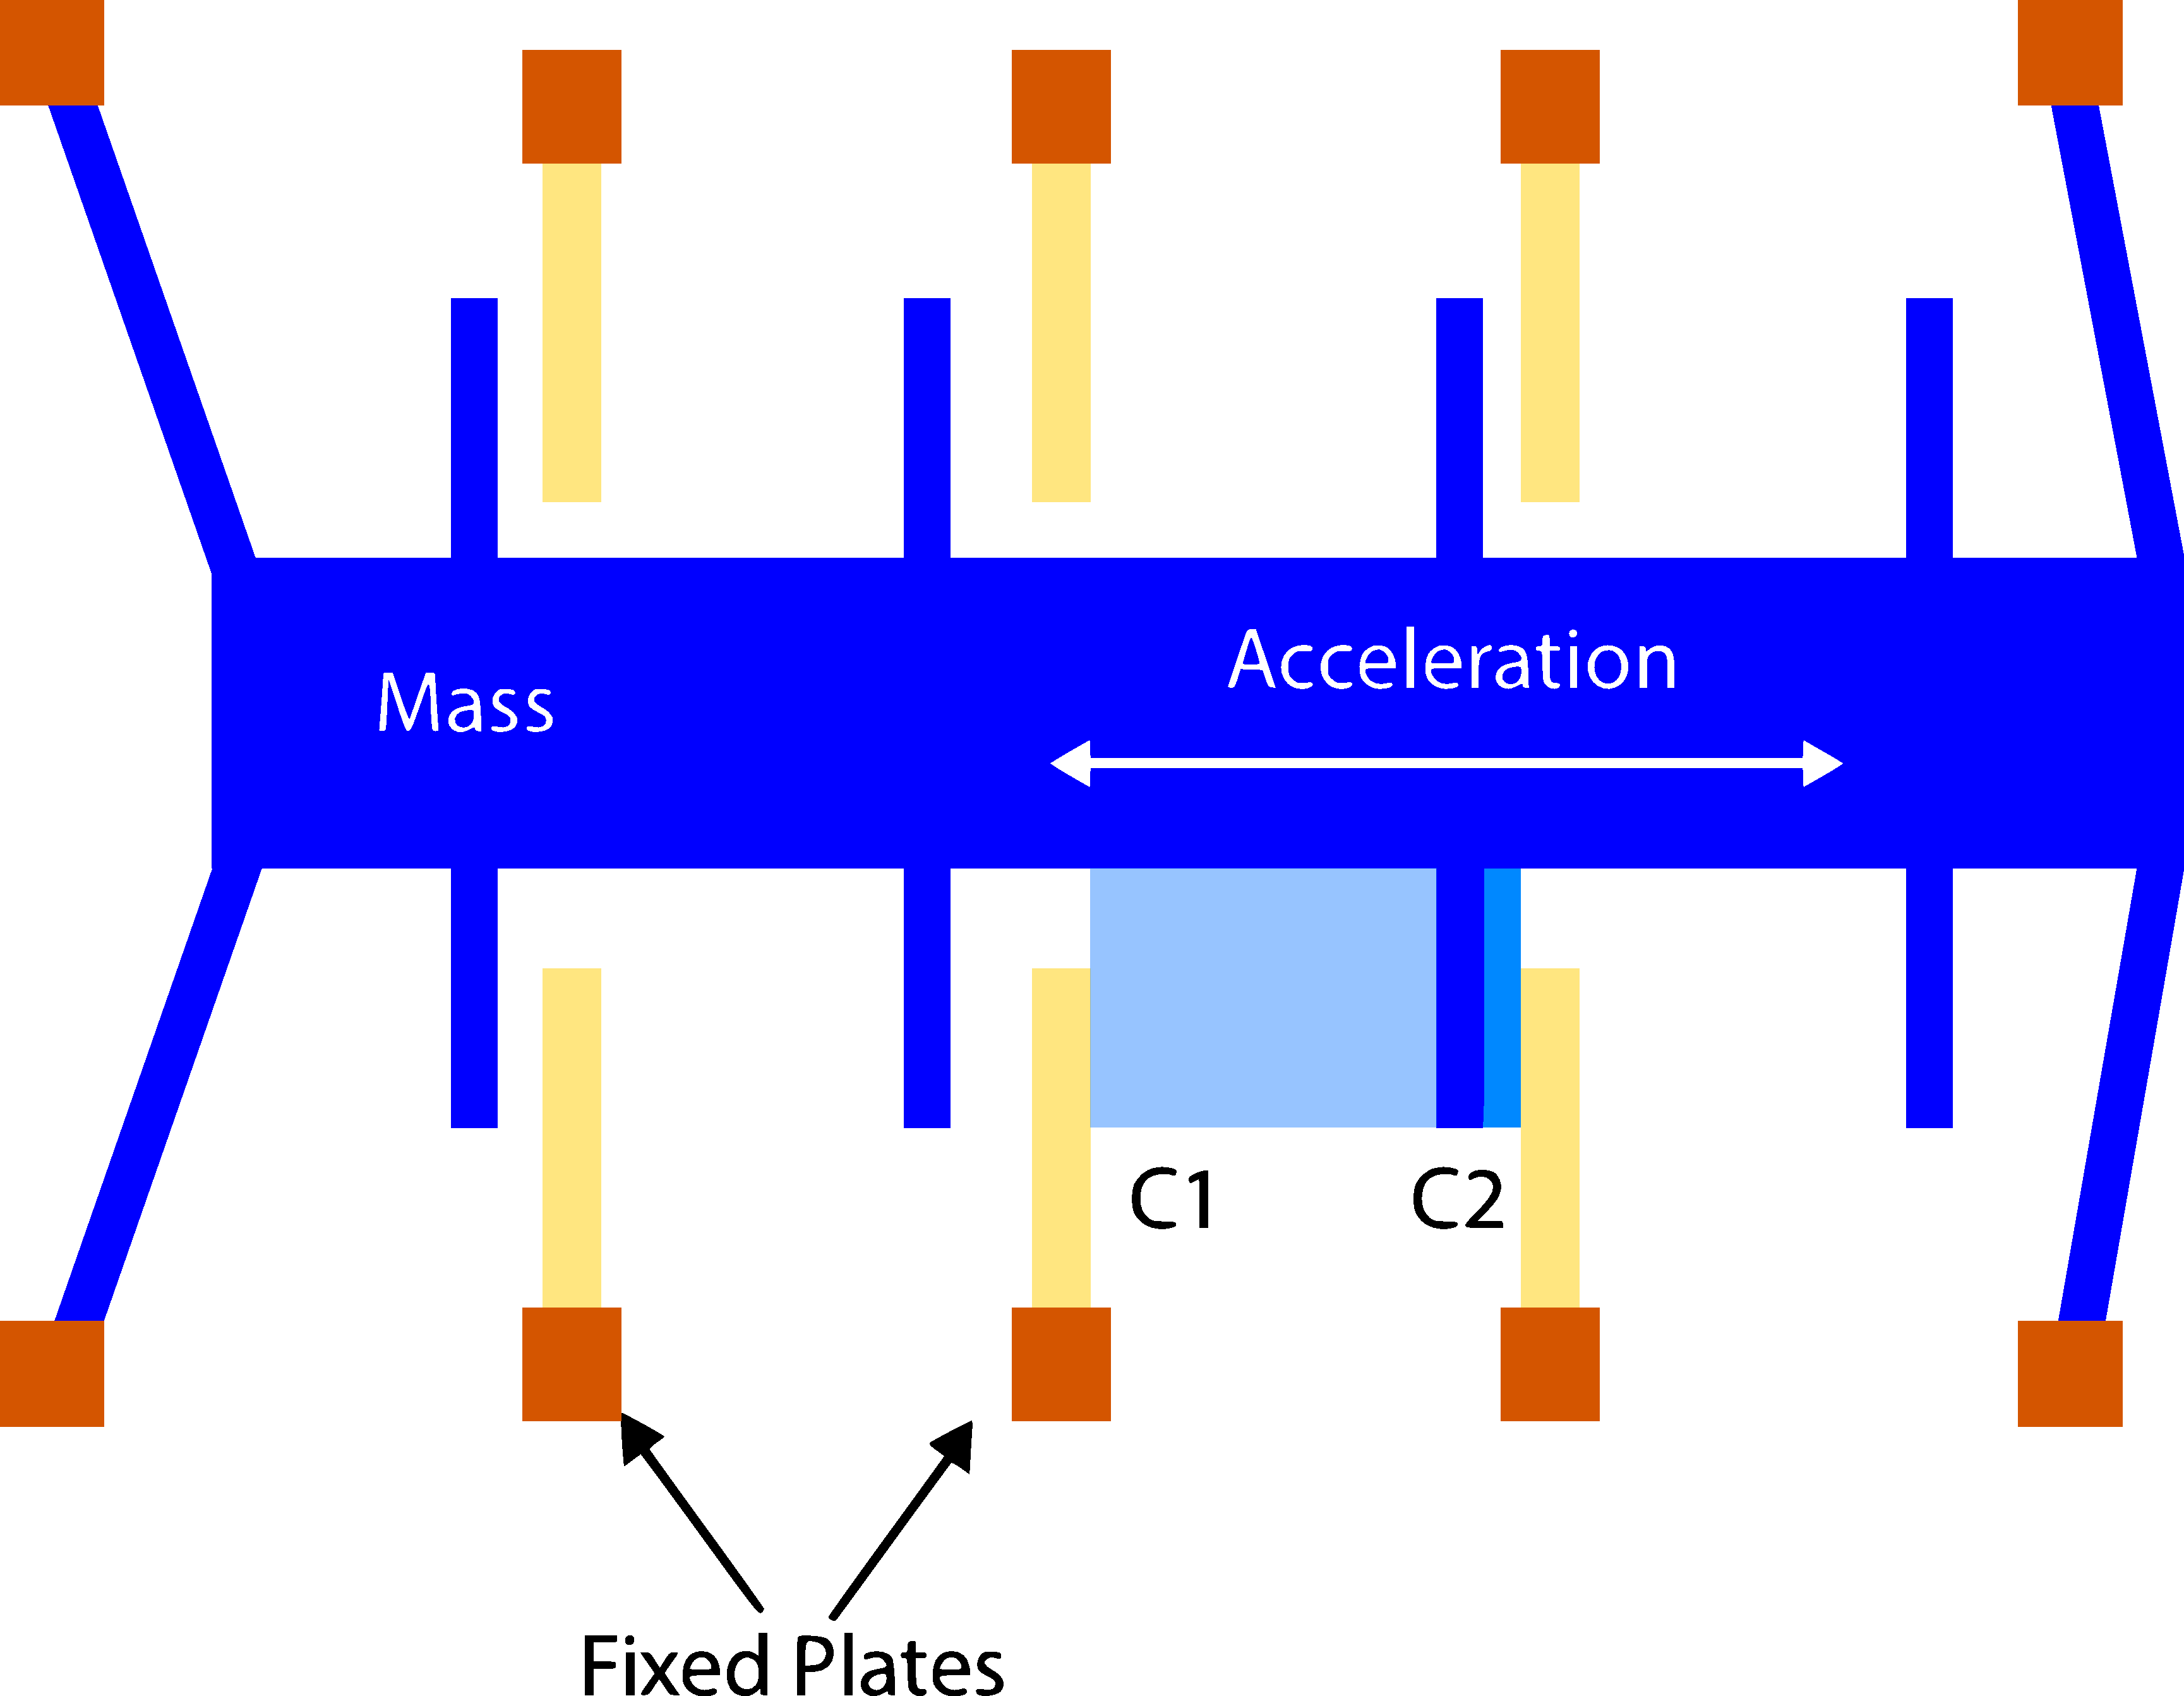
\includegraphics[width=0.2\columnwidth]{images/accelerometer_mems2.pdf}
    	}
    \end{figure}
    \scriptsize
    \begin{block}{Principio de Funcionamiento}
        Mide la aceleración midiendo el cambio en la capacitancia. Su microestructura se parece a esto. Tiene una masa unida a un resorte que se limita a moverse en una dirección y placas exteriores fijas. Entonces, cuando se aplicará una aceleración en la dirección particular, la masa se moverá y la capacitancia entre las placas y la masa cambiará. Este cambio de capacitancia será medido, procesado y corresponderá a un valor de aceleración particular.
    \end{block}
    
    \begin{itemize}
        \item Introceptivo
        \item Pasivo
        \item Mide aceleración
        \item Unidad de medición $\si{\meter\over\square\second}$
    \end{itemize}
    
\end{frame}

\begin{frame}
    \frametitle{IMU (Inertial Measurement Unit)}
    \note{página 122 del libro Introduction to autonomous mobile robots 2nd edition}
    
    \begin{itemize}
        \item 3 giróscopos ortogonales y 3 acelerómetros ortogonales.
        \item Permite estimar: posición, orientación, velocidad lineal, velocidad angular y aceleración 
        \item La orientación se obtiene integrando (con el tiempo) el giróscopo
        \item La velocidad lineal se obtiene integrando el acelerómetro
        \item La posición se obtiene integrando la velocidad
        \item Debido a que los datos del acelerómetro se integran dos veces para obtener la posición, cualquier error residual da como resultado un error cuadrático en la posición.
        \item Mediciones absolutas (GPS o cámaras) permiten cancelar esta deriva de error.
    \end{itemize}
    
    \note{
    Una unidad de medida inercial (IMU) es un dispositivo que utiliza giroscopios y acelerómetros para estimar la posición relativa, la velocidad y la aceleración de un vehículo en movimiento. Una IMU también se conoce como Sistema de Navegación Inercial (INS).
    Una IMU estima la pose de seis grados de libertad (DOF) del vehículo: posición (x, y, z) y orientación (pitch, yaw, roll). También estima velocidad y aceleración.
    
    Los datos del giroscopio se integran para estimar la orientación del vehículo, mientras que los tres acelerómetros se utilizan para estimar la aceleración instantánea del vehículo. A continuación, la aceleración se transforma en el marco de navegación local por medio de la estimación actual de la orientación del vehículo en relación con la gravedad. En este punto, el vector de gravedad se puede restar de la medición. Luego, la aceleración resultante se integra para obtener la velocidad y luego se integra nuevamente para obtener la posición, siempre que tanto la velocidad inicial como la posición sean conocidas a priori. Para superar la necesidad de conocer la velocidad inicial, la integración generalmente comienza en reposo (es decir, velocidad igual a cero).
    
    Observe que las IMU son extremadamente sensibles a los errores de medición tanto en giroscopios como en acelerómetros. Por ejemplo, la deriva en el giroscopio socava inevitablemente la estimación de la orientación del vehículo en relación con la gravedad, lo que da como resultado una cancelación incorrecta del vector de gravedad. Además, observe que, debido a que los datos del acelerómetro se integran dos veces para obtener la posición, cualquier vector de gravedad residual da como resultado un error cuadrático en la posición. Debido a esto y al hecho de que cualquier otro error se integra con el tiempo, la deriva es un problema fundamental en las IMU. Después de un largo período de funcionamiento, todas las IMU se desvían. Para cancelar esta deriva, se requiere alguna referencia a alguna medida externa.
    }
\end{frame}

